\documentclass{beamer}
\usetheme{UPJR}
\usepackage[orientation=portrait,size=a0,scale=1.4]{beamerposter}
\usepackage{fp}
\usepackage{bg}

\usepackage{xkeyval}
\usepackage{type1cm}
\usepackage{paralist}
\usepackage[spanish]{babel}
%\usepackage[latin1]{inputenc}
\usepackage[utf8]{inputenc}
\usepackage[T1]{fontenc}
\usepackage{lmodern}
\usepackage{textcomp}
\usepackage{amsmath}
\usepackage{graphicx}
\usepackage{textpos}
\usepackage{ragged2e}
\usepackage{verbatim}
\usepackage{subfigure}
\graphicspath{{graphics/}}
 \usepackage{wrapfig} %Inclusión de gráficos al lado de texto
 \usepackage[rflt]{floatflt} %Para meter figuras flotantes entre el texto
%\decimalpoint

\title{Tech-tuin}
\author{Aide Pizano Escalante, Cristian Iván Muñiz Mendoza, Elías Abraham Ramírez Rivera, José Martin Nieto León, Víctor Alfonso Humareda Barbosa}
\institute{Ingeniería en Telemática}
\footer{}
\date{}

\begin{document}
\begin{frame}[fragile]{} 
\begin{columns}[t]
  \begin{column}{0.46\textwidth}
    \begin{block}{Introducción}\justifying
      Década a década la cantidad de agua potable en México se ve disminuida debido al desperdicio inconsciente de la misma. Tan solo en Guanajuato, un habitante promedio consume alrededor de 87 litros al día, siendo aproximadamente 50 \% no reutilizable. Entre las actividades donde se presenta un mayor consumo de agua se encuentra el riego de jardines domésticos por lo que, la implementación de un sistema de riego automatizado ayuda a dar un uso más racional del agua, logrando en el proceso una mejora en la condición del jardín.\\
      \textbf{Palabras Clave:} \textit{ jardín, sistema de riego, automatización}
     \end{block}
  \end{column}
  \begin{column}{0.46\textwidth}
    \begin{block}{Objetivo}\justifying
        Desarrollar e implementar un sistema de riego automático que reduzca el consumo
agua al momento de regar jardines domésticos, utilizando un circuito electrónico que sea
capaz de tomar decisiones basado en las condiciones ambientales del jardín. \\

    \end{block}
  \end{column}
\end{columns}

\vspace*{\stretch{1}}

\justifying
\begin{columns}[t]
 \begin{column}{0.96\textwidth}
     \begin{block}{Marco Teórico}
           \vspace{0pt}
 Sistema de riego es el conjunto de estructuras que permite determinar qué área debe ser regada a partir de ciertas condiciones, aplicándole el agua necesaria a las plantas. Este consta de varios componentes. El conjunto dependerá de si se trata de riego superficial, por aspersión, o por goteo. Donde existen diferentes sistemas de riego por ejemplo:
\begin{itemize}
\item  Riego por aspersión.
\item  Riego por goteo automático
\item  Riego de superficie.
\end{itemize}
Estos riegos son manipulados manualmente por personas sin embargo, el instalar un sistema de riego tiene ventajas tales como:

\begin{itemize}

\item Se logran altos grados de automatización, basados en el ahorro de mano de obra, agua y energía.
\item Los equipos son adaptables a cualquier tipo de terreno.
\item Estos sistemas son adaptables a la rotación de plantas y a riesgos estratégicos.
\item Permite el crecimiento vertical de las plantas.

\end{itemize}
    \end{block}
  \end{column}
\end{columns}

\vspace*{\stretch{1}}

\justifying
\begin{columns}[t]
	
	
	  \begin{column}{0.46\textwidth}
	  	\begin{block}{Descripción del proyecto}
	  		\begin{minipage}[t]{1\linewidth}
	  			\vspace{0pt} 
	  			Es un sistema de riego automático que tomará decisiones para regar, con base a los datos que obtenga de los sensores, comparándolos a su vez con la información que se encuentre en la base de datos para así tomar la decisión de regar o no regar. La información de los sensores se guarda en la base de datos para tener registro de los mismos y mostrársela al usuario.
	  			\begin{figure}[H]
	  				\centering
	  				
\includegraphics[scale=0.5]{../graphics/logop}
	  			\end{figure}

			\end{minipage} 
	  	\end{block}
	  \end{column}
	
	 \begin{column}{0.46\linewidth}
	 	\begin{block}{Resultados y evidencias}
	 	De acuerdo al análisis de la investigación y la  retroalimentación, se replanteo la estructura del prototipo.
	 	\begin{figure}[H]
	 		\centering
	 		\subfigure{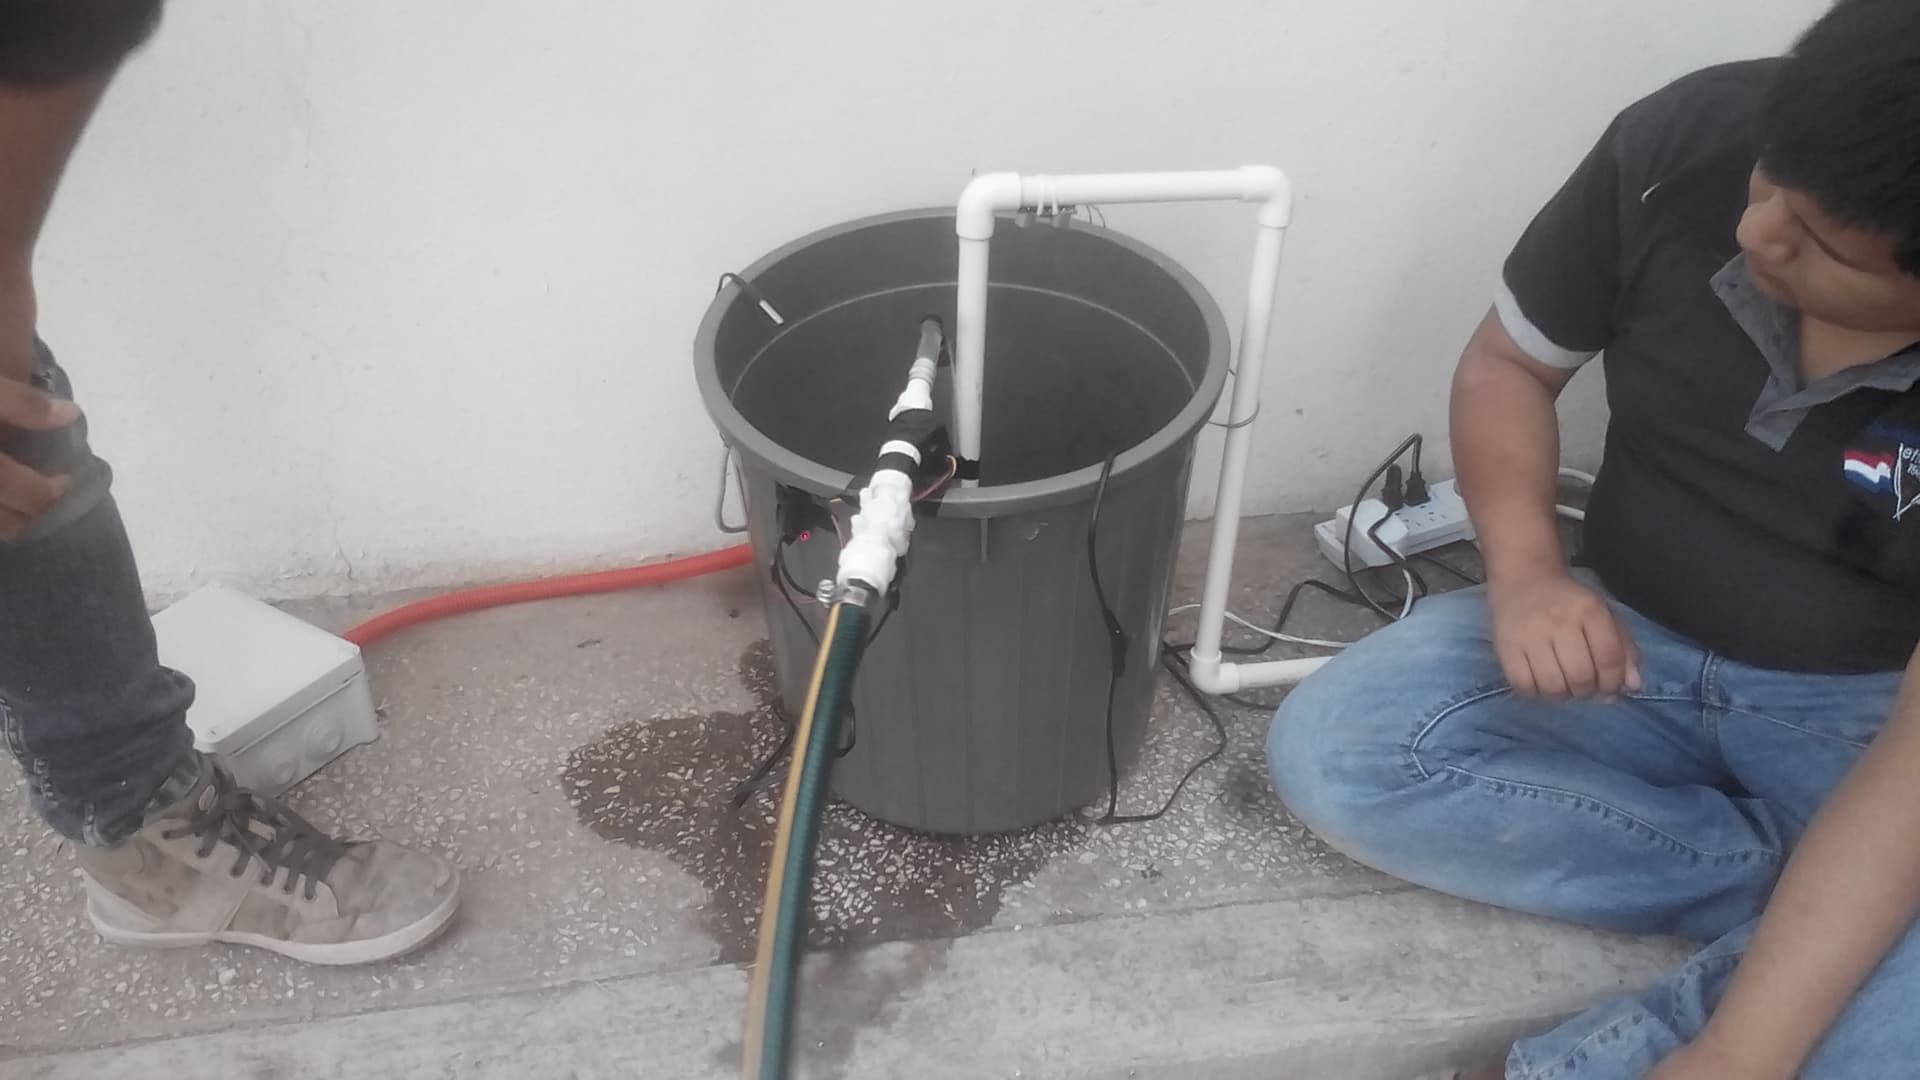
\includegraphics[scale=0.18]{../graphics/fotoq}}
	 		\subfigure{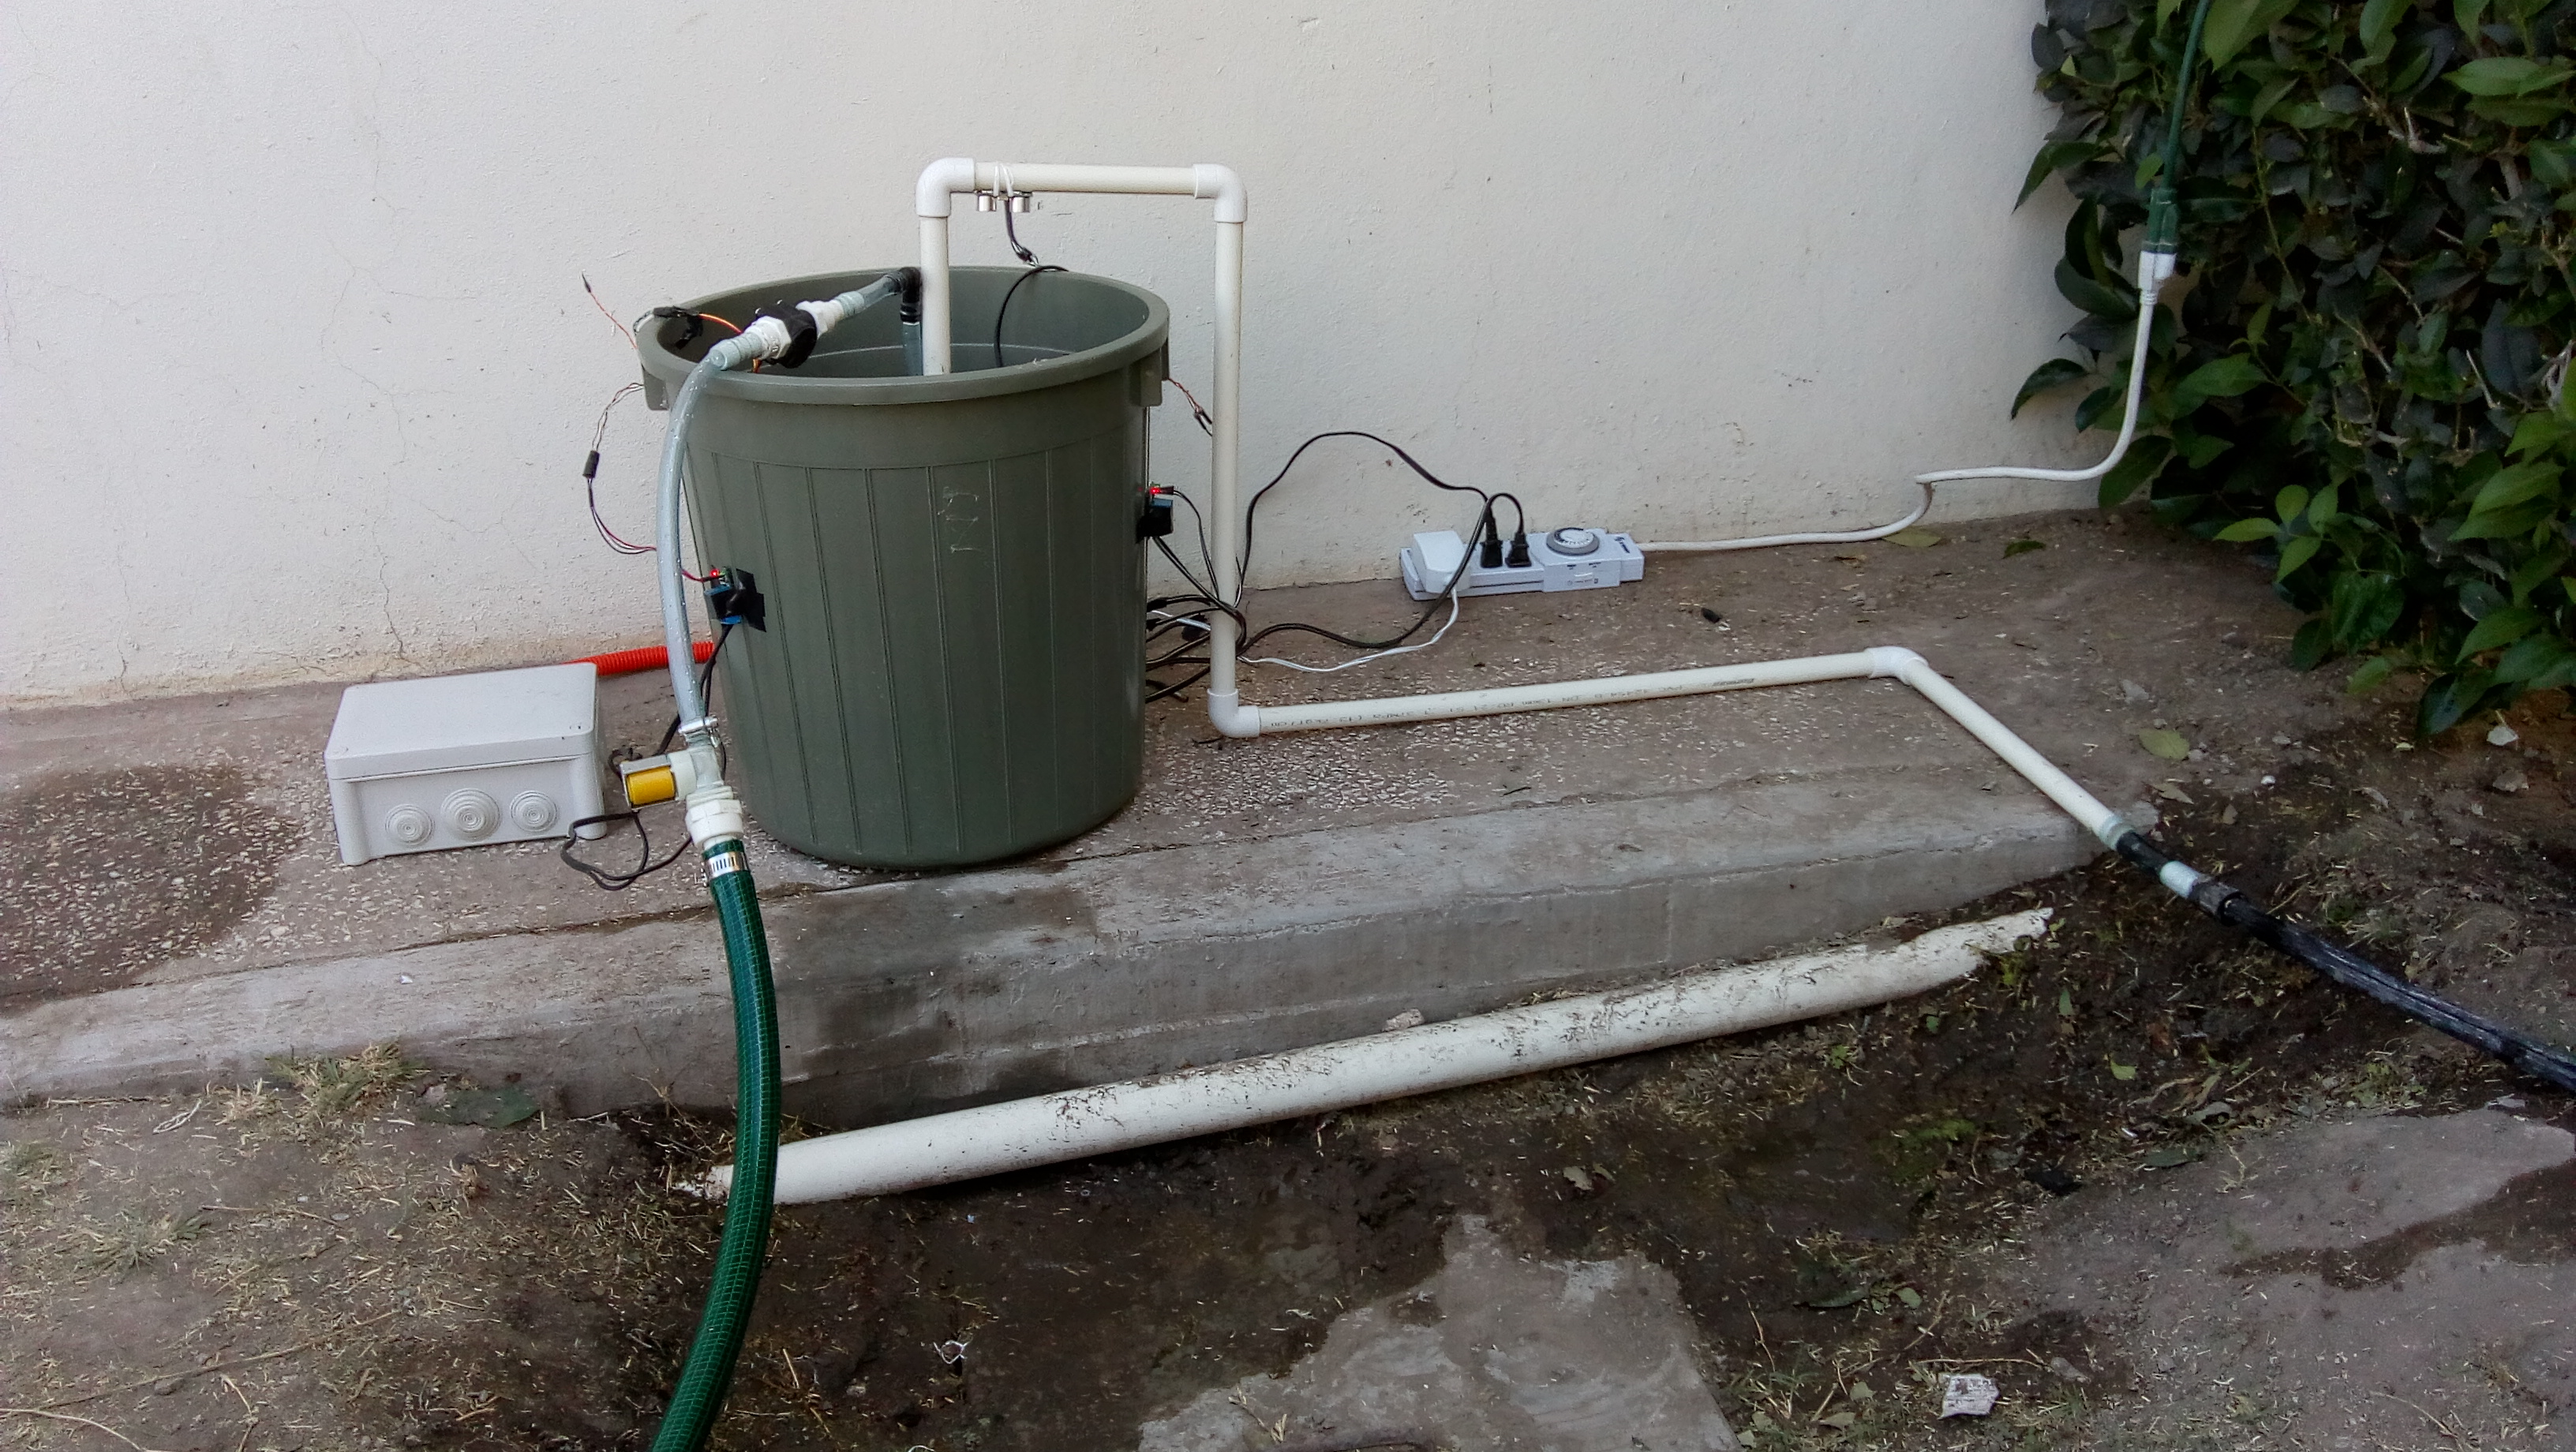
\includegraphics[scale=0.18]{../graphics/foto2}}
	 		\subfigure{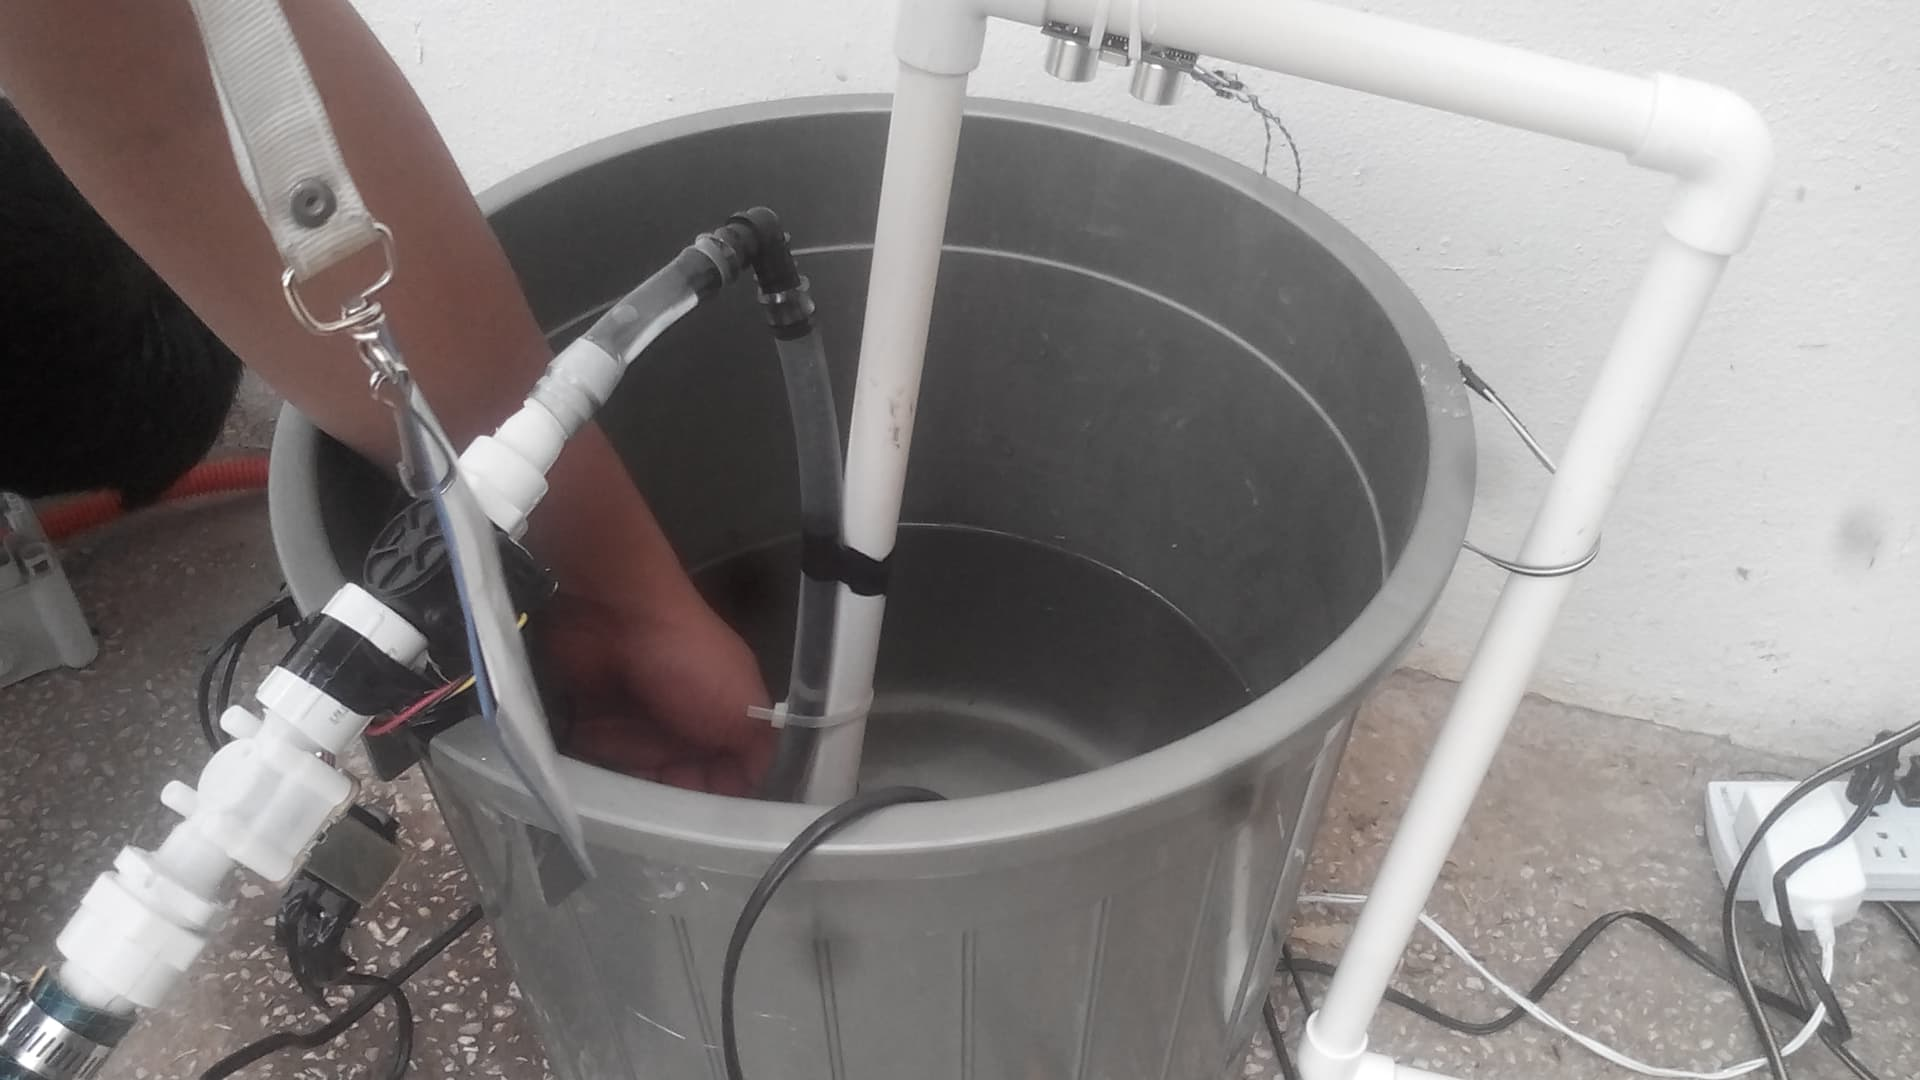
\includegraphics[scale=0.18]{../graphics/foto3}}
	 		\subfigure{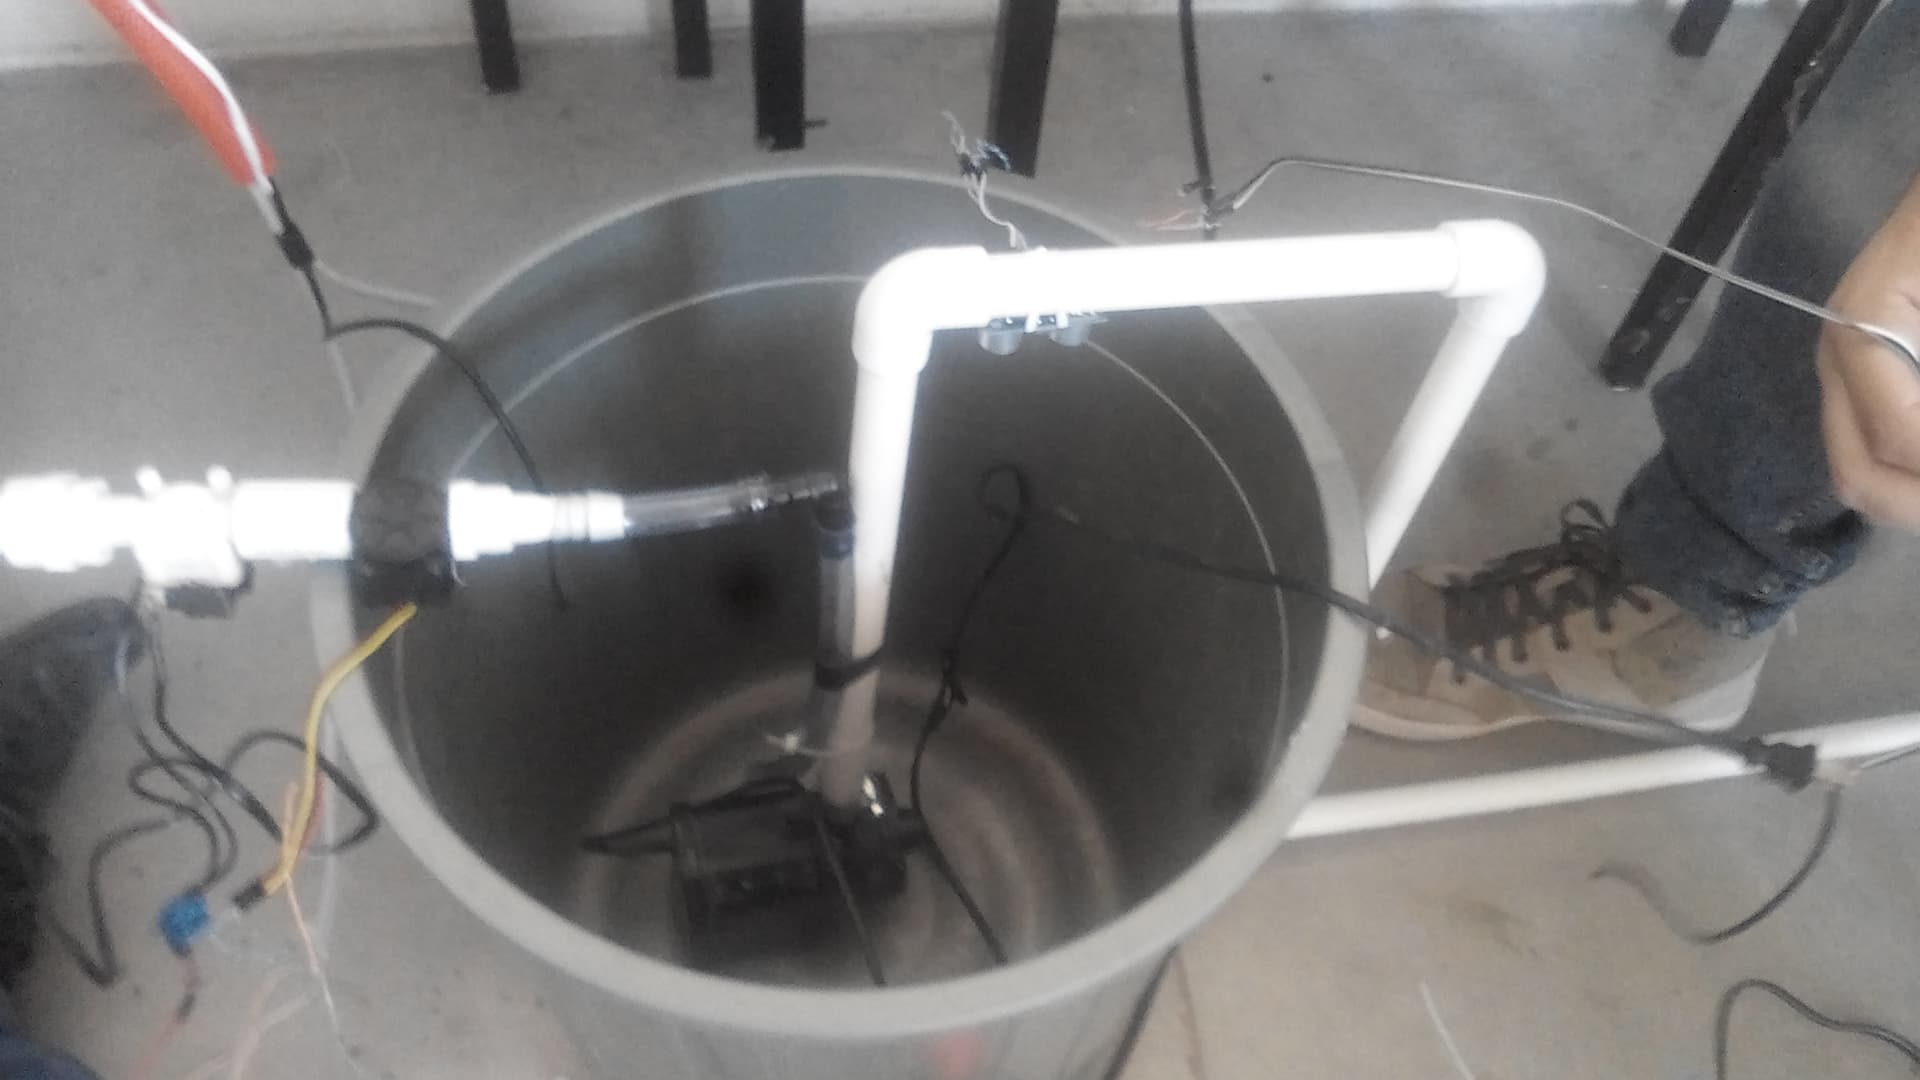
\includegraphics[scale=0.22]{../graphics/foto4}}
	 		\subfigure{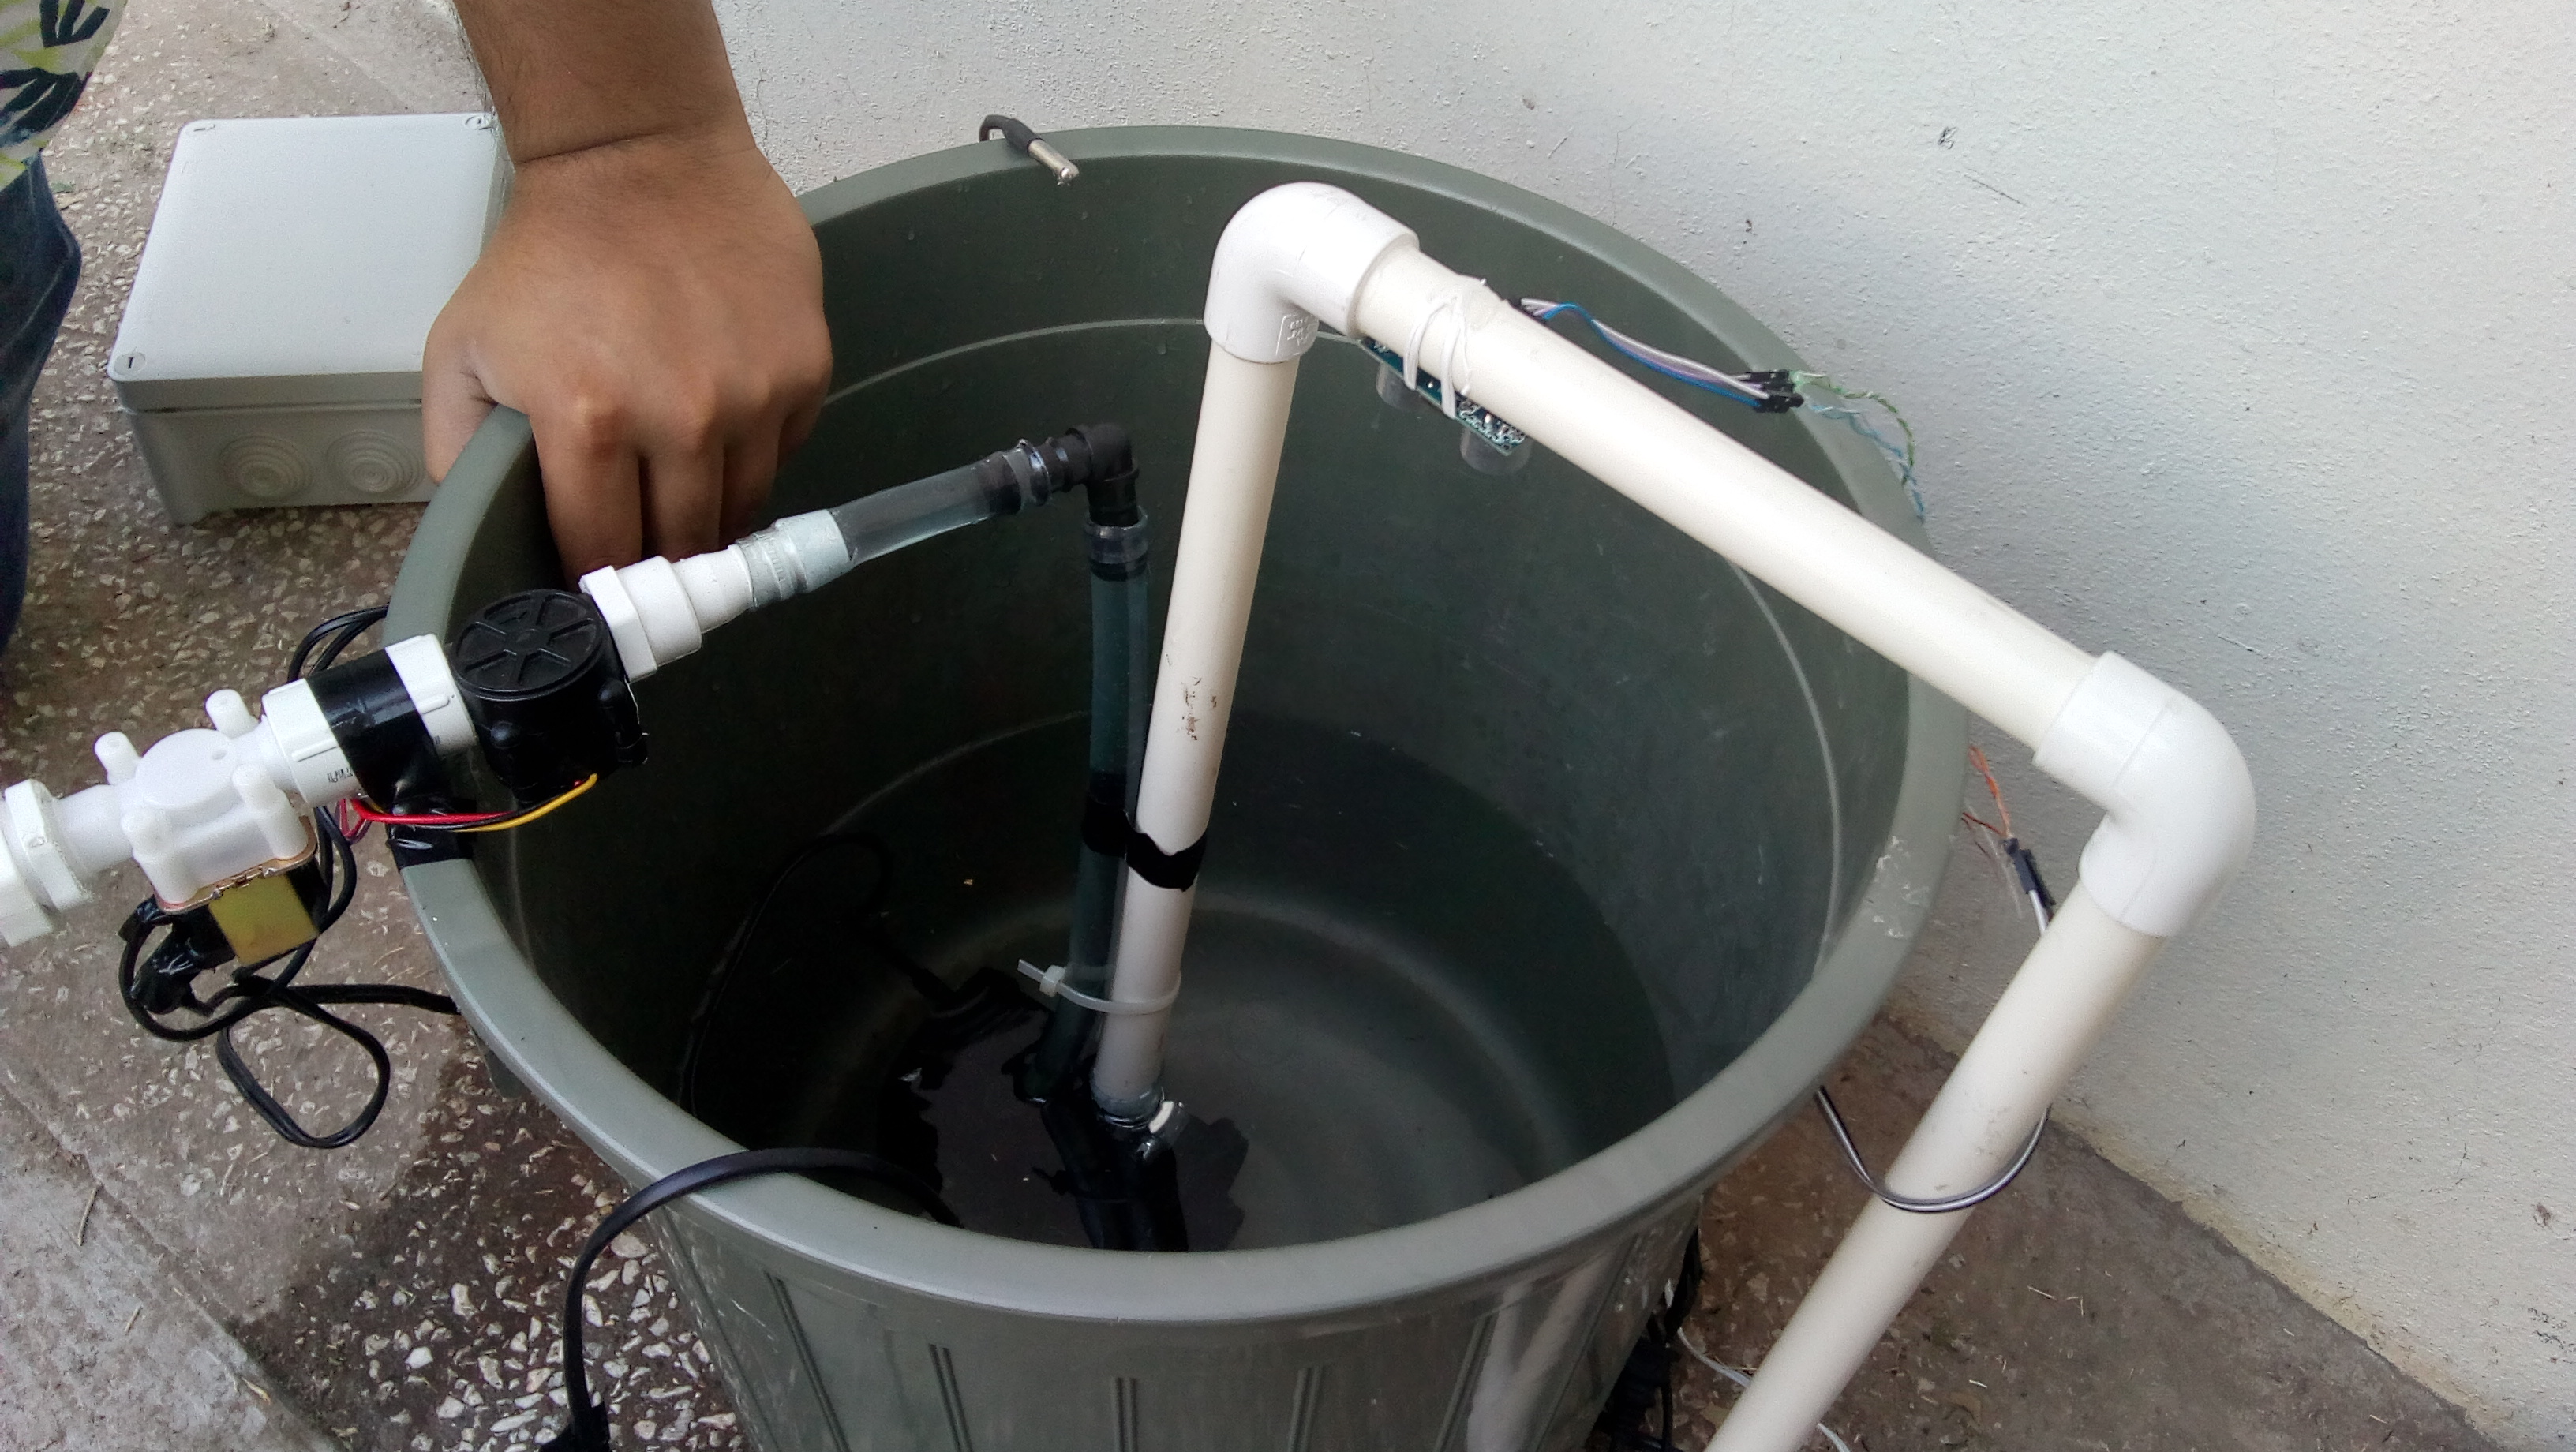
\includegraphics[scale=0.15]{../graphics/foto5}}
	 		\caption{Prototipo}
	 	\end{figure}
	 	

	 	 
	 	\end{block}
	 \end{column}
	\end{columns}
 
 	\vspace*{\stretch{1}}
 	\justifying
 	\begin{columns}[t]
 
  
  \begin{column}{0.46\linewidth}
  	\begin{block}{Trabajo a futuro}
  		\begin{minipage}[t]{1\textwidth}
  			\vspace{0pt}
 Se pretende mejorar las características de prototipo (sensores, diseño y funcionamiento) para lograr una mejor eficiencia en el desempeño del prototipo, creación de un sitio web, para mayor interacción entre producto y usuario y mejor visibilidad de datos recaudados, diseño y creación de placa PCB para circuito de electrónico.
  		\end{minipage} 
  	\end{block}
  \end{column}

	     \begin{column}{0.46\linewidth}
	     	\begin{block}{Conclusiones}\justifying
	     		\begin{minipage}[t]{0.96\textwidth}
	     			\textbf{Conclusiones}: 
	     			Durante la investigación se obtuvo que:\\
	     			Una Raspberry tiene muchas mas características que un Arduino y que serán útiles para realizar tareas como conectarse a un servidor web, multitask, administrar mas dispositivos, gestionar bases de datos, etc.
	     			\\
	     			Dos sistemas embebidos (Raspberry y Arduino) pueden comunicarse entre si utilizando medios como Wi-Fi o Bluetooth, en este caso para realizar un telemonitoreo garantizando la integridad del sistema critico.
	     			\\
	     			
	     		\end{minipage}
	     		
	     	\end{block}   
	     \end{column}
\end{columns}

\vspace*{\stretch{1}}
\justifying
\begin{columns}[t]
 \begin{column}{0.90\linewidth}
      \begin{block}{Referencias}
	\begin{minipage}[t]{0.71\textwidth}
        \begin{small}
        \begin{thebibliography}{widestlabel}
        	\bibitem{Jardinería} Gil-Albert V. F,(2006),Manual técnico de jardinería I. Establecimiento de jardines,
parques y espacios verdes, Madrid España, Mundi-prensa
        	\bibitem{arduino} Sistema de Riego Inteligente para Optimizar el Consumo de
Agua. Panama: Universidad Tecnológica de Panama.

        	\bibitem{Agricultura} Francisco Miguel Aguila Marın. (2008). Agricultura Técnica en México. Mexico: Universidad Hohenheim.
        	
        	
        	\bibitem{riego} Martín Tarjuelo. (2010). El riego y su tecnología. México: Mundi-Prensa
        	
        \end{thebibliography}
        \end{small}
        \end{minipage}
        \hfill
           \begin{minipage}[t]{0.25\textwidth}
           	\vspace{0pt}
           	\begin{center}
           		\begin{figure}
           			
\includegraphics[scale=0.2]{../graphics/ite.png} 
           		\end{figure}
           	\end{center}
           \end{minipage}
      \end{block}
   \end{column}
\end{columns}

\end{frame}
\end{document}
